\documentclass[a4paper]{article}

\usepackage[english]{babel}
\usepackage[utf8]{inputenc}
\usepackage{listings}
\usepackage{amsmath}

\usepackage{dcolumn}
\usepackage{booktabs}
\usepackage{tikz}
\usepackage{graphicx}

\usepackage{dcolumn}
\usepackage{booktabs}
\usepackage{tikz}
\usepackage{graphicx}

\usetikzlibrary{positioning,shapes,arrows}

\newcolumntype{M}[1]{D{.}{.}{1.#1}}

\title{Exercise Sheet 6}
\begin{document}
\maketitle

\section*{Problem 6.1}
\begin{itemize}
    \item
        day $d$, Moody is in state $H_d$ (happy) or $B_d$ (bad mood)
    \item
        $P(B_{d+1} | B_d) = 0.7$, $P(H_{d+1} | H_d) = 0.85$
    \item
        $P(J_d | H_d) = 0.7$, $P(DM_d | B_d) = 0.6$
    \item
        $H_0$, $DM_{1:3}$, $J_4$
\end{itemize}
1.)
\begin{align*}
    P(DM_{1:3} | H_0) = \sum_{x_1 \in \{B_1, H_1\}} &\sum_{x_{2} \in \{B_2, H_2\}} \sum_{x_{3} \in \{B_3, H_3\}} P(x_1| H_0) \cdot P(DM_1| x_1) \\
    &\cdot P(x_2| x_1) \cdot P(DM_2| x_2) \cdot P(x_3| x_2) \cdot P(DM_3| x_3)
\end{align*}

\begin{tabular}{ccccc}
    $x_0$ & $x_1$ & $x_2$ & $x_3$ & probability inside sum\\\hline
    H &  H & H & H & 0.039304000000000006\\\hline
    H & H & H & B & 0.010404\\\hline
    H & H & B & H & 0.0036720000000000004\\\hline
    H & H & B & B & 0.012852\\\hline
    H & B & H & H & 0.0036720000000000004\\\hline
    H & B & H & B & 0.000972\\\hline
    H & B & B & H & 0.004536\\\hline
    H & B & B & B & 0.015875999999999998\\\hline
\end{tabular}

Overall probability: $91.288\%$

2.)
\begin{align*}
    P(S_0) &= \langle 1, 0 \rangle\\
    P(S_1) &= \langle 0.85, 0.15 \rangle\\
    P(S_1 | DM_1) &= \langle 0.791, 0.209 \rangle\\
    P(S_2 | DM_1) &= \langle 0.735, 0.265 \rangle\\
    P(S_2 | DM_1, DM_2) &=  \langle 0.649, 0.351 \rangle\\
    P(S_3 | DM_1, DM_2) &= \langle 0.687, 0.323 \rangle\\
    P(S_3 | DM_1, DM_2, DM_3) &= \langle 0.586, 0.414 \rangle\\
    P(S_4 | DM_1, DM_2, DM_3) &= \langle 0.622, 0.378 \rangle\\
    P(S_4 | DM_1, DM_2, DM_3, J_4) &= \langle 0.794, 0.206 \rangle\\
\end{align*}

He's happy with a probability of $79.4 \%$

\section*{Problem 6.2}

1.)

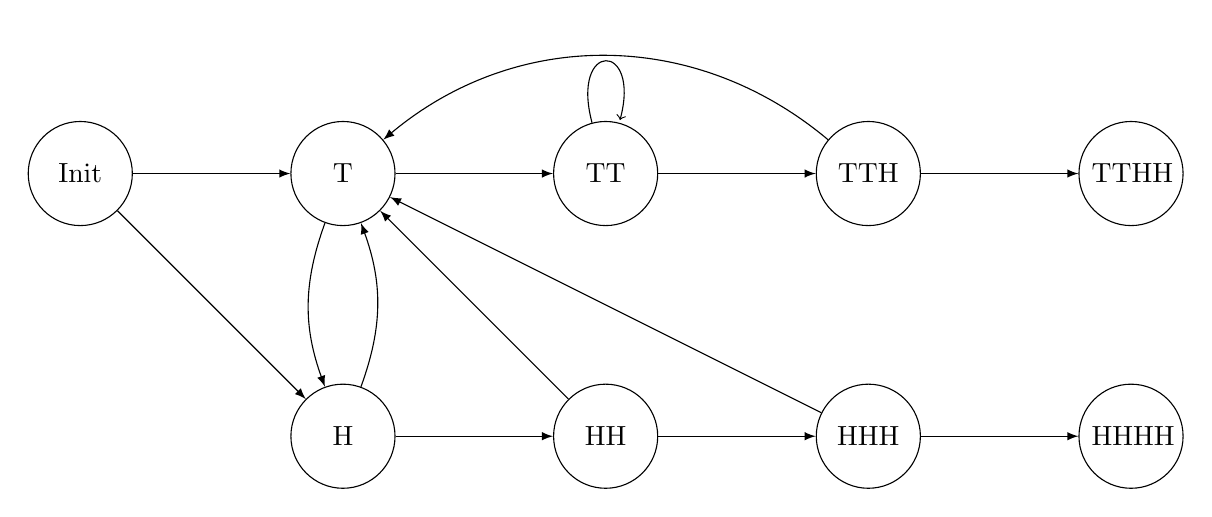
\begin{tikzpicture}[
  node distance=2cm and 2cm,
  mynode/.style={draw,circle,text width=1cm,align=center},
]

\node[mynode] (t) {T};
\node[mynode,right=of t] (tt) {TT};
\node[mynode,right=of tt] (tth) {TTH};
\node[mynode,right=of tth] (tthh) {TTHH};

\node[mynode,below=of t] (h) {H};
\node[mynode,right=of h] (hh) {HH};
\node[mynode,right=of hh] (hhh) {HHH};
\node[mynode,right=of hhh] (hhhh) {HHHH};
\node[mynode, left=of t] (empty) {Init};

\path (t) edge[-latex] (tt)
(tt) edge[-latex] (tth)
(tth) edge[-latex] (tthh)
(h) edge[-latex] (hh)
(hh) edge[-latex] (hhh)
(hhh) edge[-latex] (hhhh)
(t) edge[bend right = 20, -latex] (h)
(h) edge[bend right = 20, -latex] (t)
(hh) edge[-latex] (t)
(hhh) edge[-latex] (t)
(tt) edge[loop above, -latex] (tt)
(tth) edge[bend right=40, -latex] (t)

(empty) edge[-latex] (t)
(empty) edge[-latex] (h);
\end{tikzpicture}


2.)
Python script says that the probability that Cain wins converges to $25\%$.

\end{document}
